\section{Interfata de administrare pentru sistemul de jurnalizare}

Interfata de administrare pentru modulul de jurnalizare permite urmarirea
tuturor modificarilor care s-au facut asura datelor din baza de date.
In general, modificarile unul element al arhivei afecteaza mai multe
tabele in acelasi timp. Modificarile sunt de regula parte dintr-o
tranzactie. In sistemul de jurnalizare, fiecare tranzactie este reprezentata
printr-o revizie. O revizie este in principiu alcatuita din unul su
mai multe tabele afectate iar fiecare tabel este compus din una sau
mai multe inregistrari afectate de modificari. Fiecare rand este alcatuit
din mai multe campuri modificate. 

O baza de date in plina functionare poate atinge mii de astfel de
modificari pe zi. De aceea, identificarea unei anumite modificari
poate fi complicata. Interfata permite gruparea modificarilor atat
dupa revizii (varianta cea mai naturala) cat si dupa obiectele modificate,
utilizatorii care au facut modificarea sau ziua in care a fost facuta
modificarea. Modificarile afisate sunt aceleasi dar sunt privite din
directii diferite. 

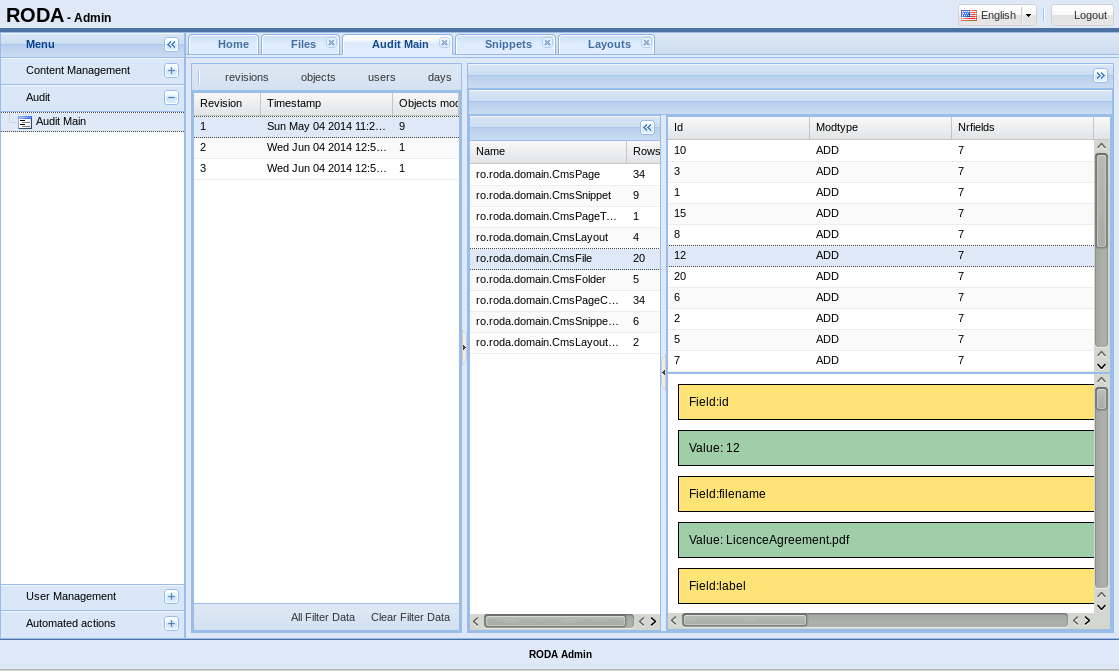
\includegraphics[width=15cm]{audit/audit1}

In figura anterioara se observa ecranul principal, cu modificarile
grupate dupa revizie. Se vede ca revizia selectata a afectat mai multe
tabele (9). Lista tabelelor afectate se obtine prin selectarea reviziei
propriu-zise. In panoul central se vede lista obiectelor (tabelelor)
modificate impreuna cu numarul de randuri afectate de modificari.
Tabelul selectat este tabelul in care sunt stocate referintele catre
fisierele stocate in zona CMS si se vede ca au fost afectate 20 de
randuri din acest tabel. Lista randurilor afectate se vede in panoul
din dreapta, partea superioara. Pentru fiecare rand se poate vedea
in lista id-ul unic al acestuia, tipul modificarii (ADD inseamna ca
randul a fost inserat in baza de date) si numarul de campuri afectate.
Lista campurilor si modificarilor aduse acestora se vede in partea
de jos a panoului din dreapta. Se observa de exemplu ca valoarea campului
filename a devenit ``LicenceAgreement.pdf''.

Ecranul contine multa informatie si in functie de tipul de modificare
facuta poate sa fie nevoie ca anumite panouri sa devina mai mari sau
altele sa fie minimizate. Ca la toate celelalte ecrane din interfata
de administrare a RODA acest lucru este posibil si se pot alcatui
mai multe configuratii de ecran. 

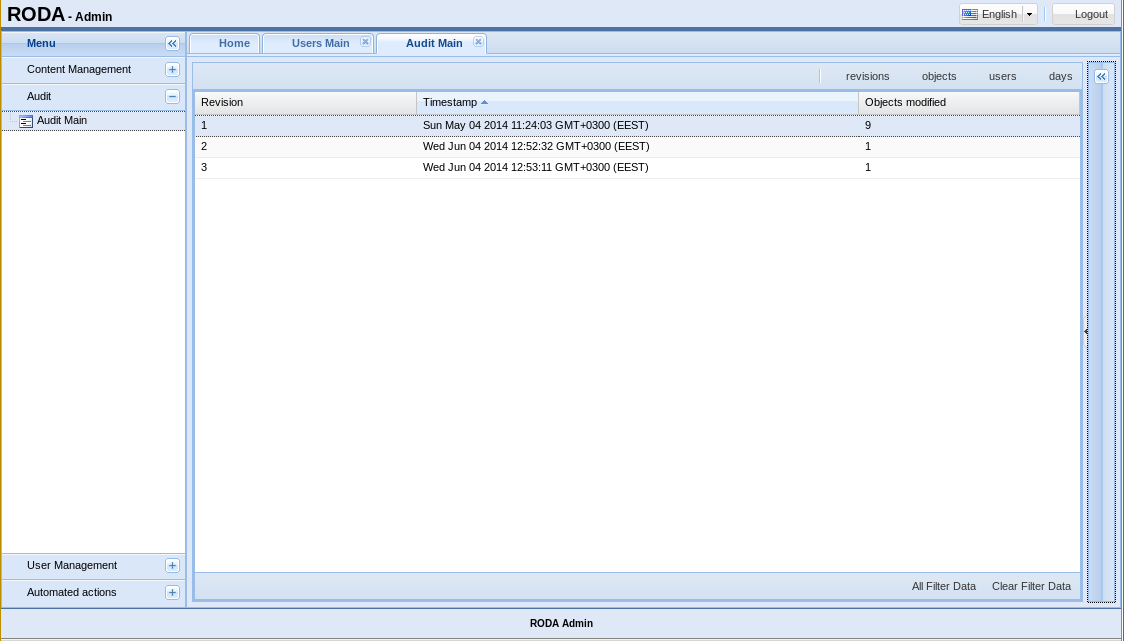
\includegraphics[width=15cm]{audit/audit2}

In imaginea anterioara au fost minimizate toate panourile care afisau
detalii cu privire la revizia curenta. In ecranul urmator se vad doar
lista reviziilor si lista campurilor modificate.

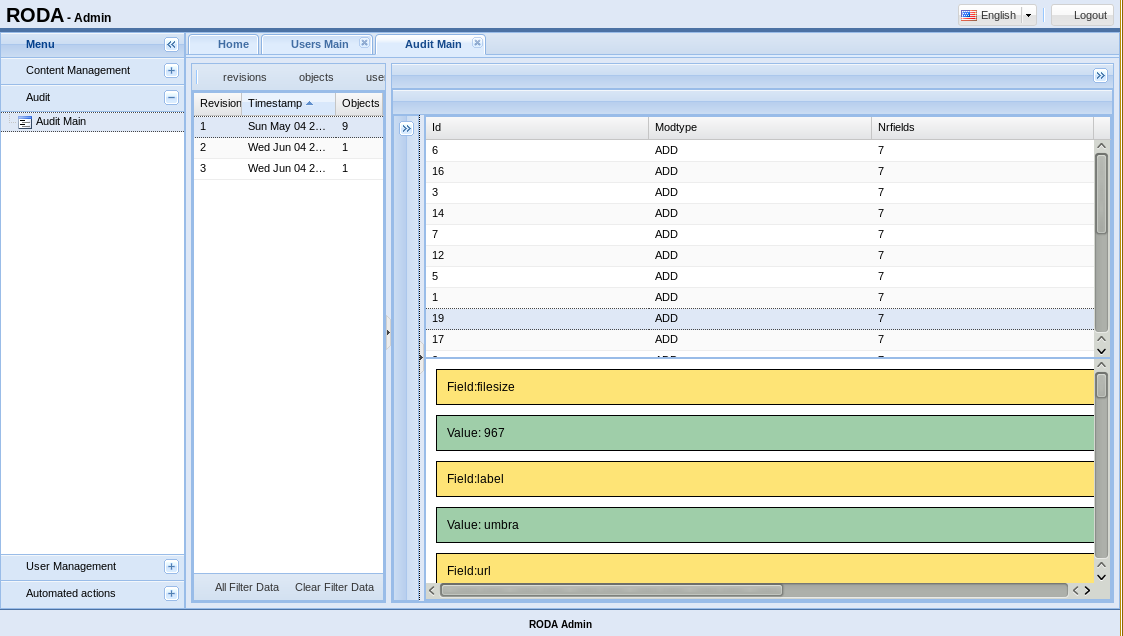
\includegraphics[width=15cm]{audit/audit3}

In figura urmatoare este prezentat acelasi ecran de audit insa cu
o perspectiva diferita - cea a obiectelor modificate:

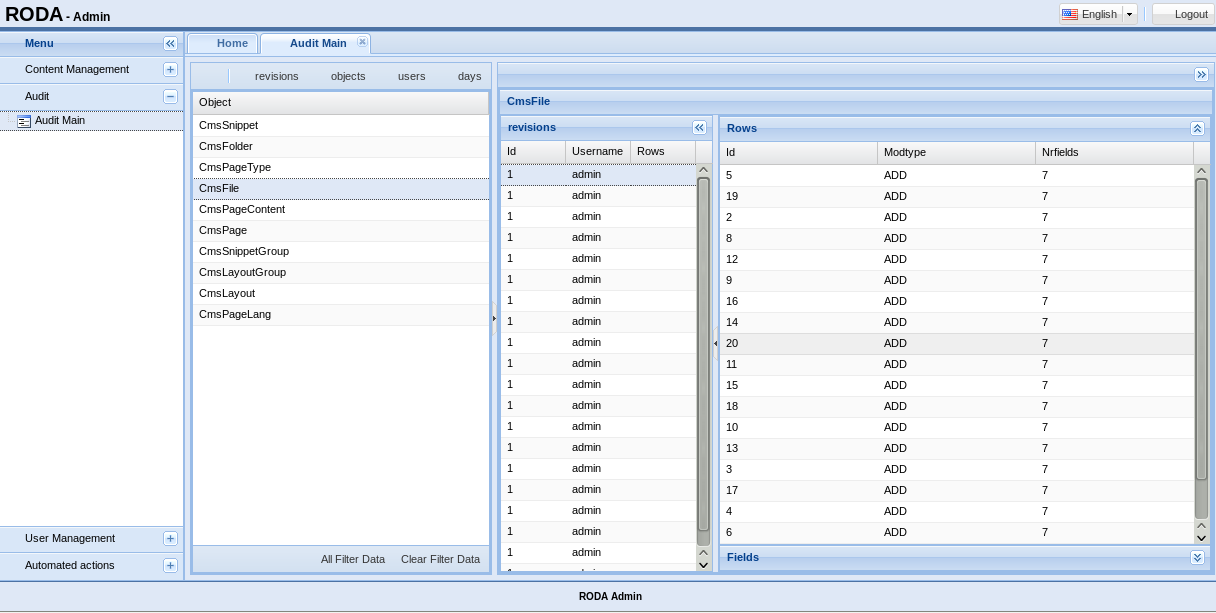
\includegraphics[width=15cm]{audit/audit4}

Se observa cum lista principala de revizii a fost inlocuita cu o lista
de obiecte. In partea dreapta se observa o lista de revizii corespunzatoare
obiectului CmsFile iar apoi lista randurilor modificate in revizia
selectata. 

